\documentclass[preprint,11pt,authoryear]{elsarticle}

\usepackage{amsmath}
\usepackage{amssymb}
\usepackage{graphicx}
\usepackage{booktabs}
\usepackage{longtable}
\usepackage[hidelinks]{hyperref}

\journal{Expert Systems with Applications}

\begin{document}

\begin{frontmatter}

\title{Self-referential performance assessment hides search degradation: a diagnostic, and a portfolio-selection case study}

\author[label1]{Víctor Adrián Sosa Hernández\corref{cor1}}
\author[label1]{Raúl Monroy Borja}
\author[label1]{Samuel Guadalupe Rodríguez Rodríguez}
\cortext[cor1]{Corresponding author.}
\affiliation[label1]{organization={«TO BE SUPPLIED»}}

\begin{abstract}
Intelligent decision-support systems built on multi-objective optimisation are routinely validated with indicators computed against a reference front produced by the same optimiser under a larger budget. We show this validation is blind by construction to any failure the two runs share, and propose one that is not: where a problem's objective extremes have a closed form, the fraction of the attainable range a front spans is measurable against ground truth.

The difference is decisive. Over 450 instances spanning 10 to 94 decision variables, the conventional indicator \emph{rises} with problem size, from 0.945 to 0.964, suggesting large instances are solved as completely as small ones. Our diagnostic \emph{falls}, from 61.3\% to 10.2\% of the attainable return range and 34.0\% to 4.3\% of the risk range, with Spearman rho = -0.93: the search degrades sharply with dimension, and the standard indicator reports the opposite.

We apply it to a screening-plus-optimisation system for equity portfolio selection on an emerging market: 6 screening arms, including gradient boosting and a tabular foundation model, over 18 monthly blocks against deterministic, index and published baselines. The diagnostic separates two claims usually made together: preselection does reduce search difficulty, and it does not improve the portfolio. No screening arm beats passing the whole universe to the optimiser, and return attribution locates the cause in a negative selection component. A mixed model over 21,275 cell-months also understates standard errors 6- to 9-fold against block resampling. Every artefact regenerates offline from a cached dataset of record.
\end{abstract}

\begin{highlights}
\item Reference-front indicators cannot detect search failures the reference shares
  \item Coverage against closed-form extremes measures front quality on ground truth
  \item Coverage falls from 61.3\% to 10.2\% as size grows
  \item Preselection eases the search yet still lowers portfolio return
  \item Block-paired tests replace a mixed model that overstates precision 9-fold
\end{highlights}

\begin{keyword}
Multi-objective optimisation; performance assessment; evolutionary computation; portfolio selection; machine learning screening; reproducibility
\end{keyword}

\end{frontmatter}

% --- introduction --------------------------------------------------------
\section{Introduction}\label{sec:introduction}

A decision-support system built on multi-objective optimisation presents its user with a set of trade-offs rather than a single answer, and the value of the system rests on that set being a fair picture of what is achievable. Validating it is therefore a question about the produced front, not about the objective values of any one solution, and the field answers that question with indicators: hypervolume, inverted generational distance, attainment. Each requires something to compare against.

On synthetic benchmarks the comparison is exact, because the true front is known by construction. In an application it is not known, and practice substitutes a reference front assembled from the algorithms under study -- commonly the same algorithm run under a larger budget. The substitution is treated as a practical necessity with no consequences for what the indicator means.

This paper shows the consequence is real and can invert a conclusion. A reference front produced by the same optimiser inherits whatever that optimiser cannot reach, so an indicator computed against it reports agreement between two runs rather than quality. Where the search systematically fails to reach part of the objective space, both runs fail the same way, the indicator sees nothing, and the system passes validation while presenting its user with a fraction of the available trade-offs.

We make the failure measurable. For problems whose objective extremes have a closed form -- which includes the constrained mean-variance formulation and any problem where a linear objective is optimised over a simplex -- the attainable range can be computed rather than estimated, and the fraction of it a front spans is a quantity no shared bias can move. We call it coverage, give the condition under which a reported attainment is untrustworthy, and show that on our problem the two measures disagree in direction across the full range of problem sizes tested.

The setting is a screening-plus-optimisation system for equity portfolio selection: a supervised classifier admits or rejects candidate instruments, and a multi-objective optimiser allocates over what survives. This architecture is common, and the preselection step is justified on two grounds that are usually asserted together -- that it improves the portfolio, and that it makes the optimisation tractable by reducing decision variables. Our diagnostic separates them, and they come apart: the tractability claim holds and the quality claim fails.

Section headings below follow the order in which the argument is built. We state the diagnostic and its guard condition, describe the system and the evaluation protocol, report what both measures say about problem size, report the system's own performance against deterministic, index and published comparators, and close with what the design can and cannot resolve.


% --- contributions -------------------------------------------------------
\section{Contributions}\label{sec:contributions}

\textbf{An indicator that cannot see its own failure mode, and a correction.} Attainment computed against an extended-budget reference front rises with problem size on our ablation, from 0.945 at 10 decision variables to 0.964 at 94. Measured against the closed-form attainable range instead, coverage of the reachable return range falls from 61.3\% to 10.2\% and of the risk range from 34.0\% to 4.3\%, with Spearman rho = -0.93 over 75 instances. The two readings are contradictory and only one is checkable against ground truth. We give the coverage measure, a guard that refuses to report attainment without it, and the condition that flags the pathology: high attainment beside low coverage.

\textbf{A demonstration that this changes a substantive conclusion.} The ablation was designed to test whether supervised preselection earns its place. On the attainment reading it does not, on any axis. On the coverage reading the tractability claim holds and the quality claim still fails: preselection genuinely makes the search easier, and separately, the screening signal is bad enough that the easier search does not pay for it. Those are separable findings, and an indicator that conflates them would have suppressed one.

\textbf{An inferential hazard in blocked experimental designs.} Fitting a mixed model over 21,275 cell-months with the block as a random effect yields standard errors 6 to 9 times smaller than resampling whole blocks. The point estimates agree exactly; only the precision differs. A random intercept removes a block's common level but not the cross-sectional dependence among configurations that share underlying data, so the model treats correlated cells as replicates. We report both and let the pre-registered block-paired tests govern.

\textbf{A negative empirical result, reported in full.} Across 6 screening arms over 18 monthly blocks, none beats passing the whole admitted universe to the optimiser: 12.0\% annualised for the no-screening control against 7.9\% for the best arm and 0.1\% for the worst, at 50 basis points. Return attribution isolates the mechanism -- the selection component is negative for every screening arm, between -7.3\% and -3.1\%, and exactly zero for the control, which validates the decomposition. No effect exceeds the design's detectable bound of 12.7\% to 17.1\%, so these are reported as unresolved rather than as null.

\textbf{A replication package.} The pipeline is specified before execution, runs from a cached dataset of record with the network unavailable, and regenerates every table, figure and quoted number. Configuration drift is detectable: seeds derive from a configuration fingerprint that is checked against the manifest, a property added after the drift occurred undetected during development.


% --- related_work --------------------------------------------------------
\section{Related work}\label{sec:related-work}

\textbf{Performance assessment in multi-objective optimisation.} The hypervolume indicator \citep{zitzler1999} and the attainment function \citep{fonseca1996} are the standard instruments for comparing stochastic multi-objective optimisers, and both require a point of comparison. Where the true Pareto front is known -- on synthetic benchmarks constructed for the purpose -- that point is exact. Where it is not, which is every real application, practice substitutes a reference front assembled from the algorithms under study, often from an extended-budget run of the same algorithm. The substitution is usually described as a practical necessity and treated as benign.

This paper is about a case where it is not benign. A reference front produced by the same optimiser inherits whatever that optimiser cannot do, so an indicator computed against it measures consistency rather than quality, and reports success precisely when the failure is systematic. The problem is distinct from the well-studied sensitivity of hypervolume to its reference point, which concerns the scaling of a comparison rather than its blindness.

\textbf{Statistical comparison across problems.} Comparing optimisers over multiple problem instances is conventionally handled with rank-based tests and critical-difference diagrams \citep{demsar2006}. We use that machinery and report the interval it implies, because over a small number of blocks the interval is wide enough that adjacency in such a diagram carries almost no information -- a property of the design that a diagram without its interval invites readers to ignore.

\textbf{Portfolio selection as a multi-objective problem.} The mean-variance formulation \citep{markowitz1952} is the canonical two-objective instance, and evolutionary approaches to it are well established; NSGA-III \citep{deb2014} is the algorithm used here. The formulation suits our purpose for a reason independent of finance: under a simplex constraint both extremes are analytic, so the attainable range is computable and the indicator can be checked against ground truth rather than against itself.

\textbf{Preselection and dimensionality reduction.} Applications commonly reduce the decision space before optimising, and supervised preselection -- training a classifier to admit or reject candidates -- is a frequent choice, justified on two grounds: that it improves the solution by removing bad candidates, and that it makes the search tractable by reducing decision variables. Our ablation tests both claims independently, and finds that they come apart.

\textbf{Comparators.} The empirical arms are placed against deterministic baselines (equal weighting, inverse volatility, minimum variance, maximum Sharpe), against the reference series an investor would hold instead -- the CETES 28-day instrument at 7.8\% annualised, the local index at 19.4\%, and the S\&P 500 converted to pesos -- and against adapted published approaches: a single-objective genetic algorithm maximising the Sharpe ratio, an L1-regularised mean-variance formulation with shrinkage covariance, and a cross-sectional momentum portfolio. Momentum is the demanding one, at 28.2\%, above every arm the studied method produces.


% --- method --------------------------------------------------------------
\section{The diagnostic}\label{sec:method}

\subsection{What a self-produced reference cannot show}

Let an optimiser produce a front $F$ on an instance, and let $R$ be a reference front produced by the same optimiser under a larger budget. Any indicator of the form $I(F, R)$ is a statement about the relationship between two samples from the same procedure. If the procedure cannot reach a region of the objective space at all, neither $F$ nor $R$ contains points there, the region is absent from the comparison, and $I(F, R)$ is unaffected by its absence. The indicator does not fail; it answers a different question than the one the analyst intends.

This matters most exactly where reassurance is most wanted. As an instance grows, a search that degrades will produce a narrower $F$ -- and a correspondingly narrower $R$. The ratio can rise while both collapse.

\subsection{Coverage against a computable bound}

Where the extremes of each objective can be computed in closed form, the comparison need not be self-referential. For the constrained mean-variance problem over a simplex, the maximum expected return is attained by placing the whole budget on the single highest-mean asset, and the minimum variance is the analytic minimum-variance portfolio. Both are exact and neither involves the optimiser.

Writing $[\,a_j, b_j\,]$ for the attainable range of objective $j$ and $[\,\hat{a}_j, \hat{b}_j\,]$ for the range the produced front spans, coverage is

\begin{equation}
  C_j(F) \;=\; \frac{\hat{b}_j - \hat{a}_j}{b_j - a_j}.
\end{equation}

Coverage is bounded above by one, is comparable across instance sizes because it is normalised by what is attainable on each, and cannot be moved by a bias the produced and reference fronts share, because no reference front enters it.

The requirement is that the extremes be computable, not that the whole front be known. This is weaker than it first appears: it holds whenever each objective, taken alone, is optimised by a solution with a closed form, which covers linear objectives over a simplex, convex quadratic objectives with analytic minimisers, and any objective whose single-objective optimum is available from a solver the analyst already trusts.

\subsection{The guard condition}

Coverage does not replace attainment, which answers a legitimate question about budget sufficiency. It constrains how attainment may be read. We report the pair, and flag the configuration in which the two disagree in the dangerous direction: attainment at or above nine tenths beside coverage below one quarter. That combination says the search is consistent with itself and narrow against the problem, which is the signature this paper is about. A reported attainment unaccompanied by coverage is, on this evidence, not interpretable.


% --- experimental_setup --------------------------------------------------
\section{Experimental setup}\label{sec:experimental-setup}

\textbf{Market and window.} Equities on the Mexican Stock Exchange, evaluated monthly over 18 blocks from 2025-01 to 2026-06. The universe is screened point-in-time on liquidity and data quality, admitting between 88 and 101 instruments per month. Price history reaches further back than the evaluation window to supply indicator warm-up, the expanding training pool and the covariance estimate.

\textbf{Screening arms.} 6 arms, comprising a no-screening control that passes the whole admitted universe to the optimiser and machine-learning screeners spanning support vector machines, random forests, neural networks, gradient boosting and a tabular foundation model. Each is tuned by inner cross-validation on a classification metric, never on portfolio return, so the portfolio outcome stays out of sample. Three labelling strategies are crossed with the screeners.

\textbf{Optimisation.} NSGA-III on the two-objective mean-variance problem, with expected return and ex-ante risk estimated from trailing daily returns. Three portfolios are extracted from each front -- minimum risk, knee and maximum return -- and evaluated under two concentration caps, the looser of which reproduces the unconstrained formulation. Independent seeds are replicated per cell, giving 21,275 evaluated cell-months in the factorial.

\textbf{Evaluation.} Portfolios are priced on executable prices, charged round-trip transaction costs under four scenarios, and reported at 50 basis points as the primary scenario; the zero-cost scenario is reported only as an upper bound. Returns are decomposed into market, selection, allocation and a currency tilt by an identity whose residual is zero by construction, which the no-screening control exercises as an internal check.

\textbf{Comparators.} Three tiers: deterministic analytic allocators over the same universe; reference series an investor would hold instead, including the local index and the sovereign short-rate instrument; and adapted published approaches, among them a single-objective genetic algorithm on the Sharpe ratio and a cross-sectional momentum portfolio.

\textbf{Ablation.} The search-space ablation truncates each screener's ranked output to fixed sizes and adds no-preselection as an explicit level, giving 450 instances from 10 to 94 decision variables. Both attainment against an extended-budget reference and coverage against the closed-form range are recorded per instance.

\textbf{Statistical protocol.} The confirmatory hypotheses, their contrasts and their metrics are fixed before execution; everything else is labelled exploratory. Tests are paired on the evaluation block, corrected across the confirmatory family, and reported with the minimum effect the design can detect, which is 12.7\% to 17.1\% annualised. A result below that bound is reported as unresolved, never as evidence of equivalence.


% --- results -------------------------------------------------------------
\section{Results}\label{sec:results}

\subsection{The two measures disagree in direction}

Across 450 ablation instances, attainment against an extended-budget reference rises monotonically with problem size, from 0.945 at 10 decision variables to 0.964 at 94. Read alone, this says the larger instances are solved as completely as the smaller ones and that a fixed-budget comparison across sizes is sound.

Coverage says the opposite. Over 75 instances, the fraction of the attainable return range the front spans falls from 61.3\% at 10 variables to 10.2\% at 93, and the risk range from 34.0\% to 4.3\%. The rank correlation between problem size and return coverage is -0.93. Because the asset pools are nested, the attainable range can only widen with size -- and it does, while the range the optimiser spans narrows.

The effect is visible in the portfolios themselves rather than only in the indicator. On the no-screening control at the median evaluation month, the three extracted profiles hold nearly the entire universe at a maximum weight close to a thirtieth, and their expected returns differ by less than a tenth of a percentage point per month. The aggressive and conservative profiles are, in substance, the same portfolio. The concentration ratio against equal weight stays roughly constant across sizes, so the optimiser is finding structure; it is the span that collapses.

\subsection{Search cost does not grow with the problem}

Wall-clock rises from 2.1 to 4.1 seconds between 10 and 94 variables, a factor of 2.0, while the covariance matrix grows by a factor of 88. Preselection is therefore not buying computation at this scale, whatever it may buy in search quality.

\subsection{The system's own performance}

No screening arm beats the no-screening control. At 50 basis points the control returns 12.0\% annualised against 7.9\% for the best machine-learning arm, neural network, and 0.1\% for the worst, random forest. Return attribution locates the cause: the selection component is negative for every screening arm, between -7.3\% and -3.1\% annualised, while the same decomposition returns exactly zero for the control.

Against the comparator suite the ordering is unfavourable to the proposed architecture. The cross-sectional momentum portfolio returns 28.2\%, the local index 19.4\%, and the sovereign short-rate instrument 7.8\%, all above every screening arm and the first two above the control.

\subsection{Nothing separates statistically, and the design says why}

None of the confirmatory hypotheses rejects, and every estimated effect falls below the detectable bound of 12.7\% to 17.1\%. The hierarchical tests, each holding the other factors at their best level, return probabilities between 0.42 and 0.68. The critical difference over the pre-registered headline set of 6 cells is 1.78 ranks against an observed spread far smaller, so no pair is separated.

These are statements about resolution, not about equivalence, and we report them as such.

\subsection{Inference is sensitive to how dependence is handled}

Fitting a mixed model over 21,275 cell-months with the evaluation block as a random effect yields standard errors 6 to 9 times smaller than resampling whole blocks. The point estimates agree; only the precision differs. Cells within a block hold overlapping instruments and move together, and a random intercept removes the block's common level while leaving that dependence intact, so the model treats correlated configurations as replicates. The block-paired tests, named confirmatory in advance, govern; the model is reported as descriptive.

The labelling-by-allocator interaction, which is the direct test of whether an apparent labelling advantage is a concentration effect in disguise, has 10 terms and none reaches significance even at the model's overstated precision.

\subsection{Robustness}

Substituting a shrinkage covariance estimator moves the reported contrasts by at most 0.7\% annualised, and no contrast reverses sign. The estimator is therefore not promoted to a design factor.

\begin{figure}[htbp]
  \centering
  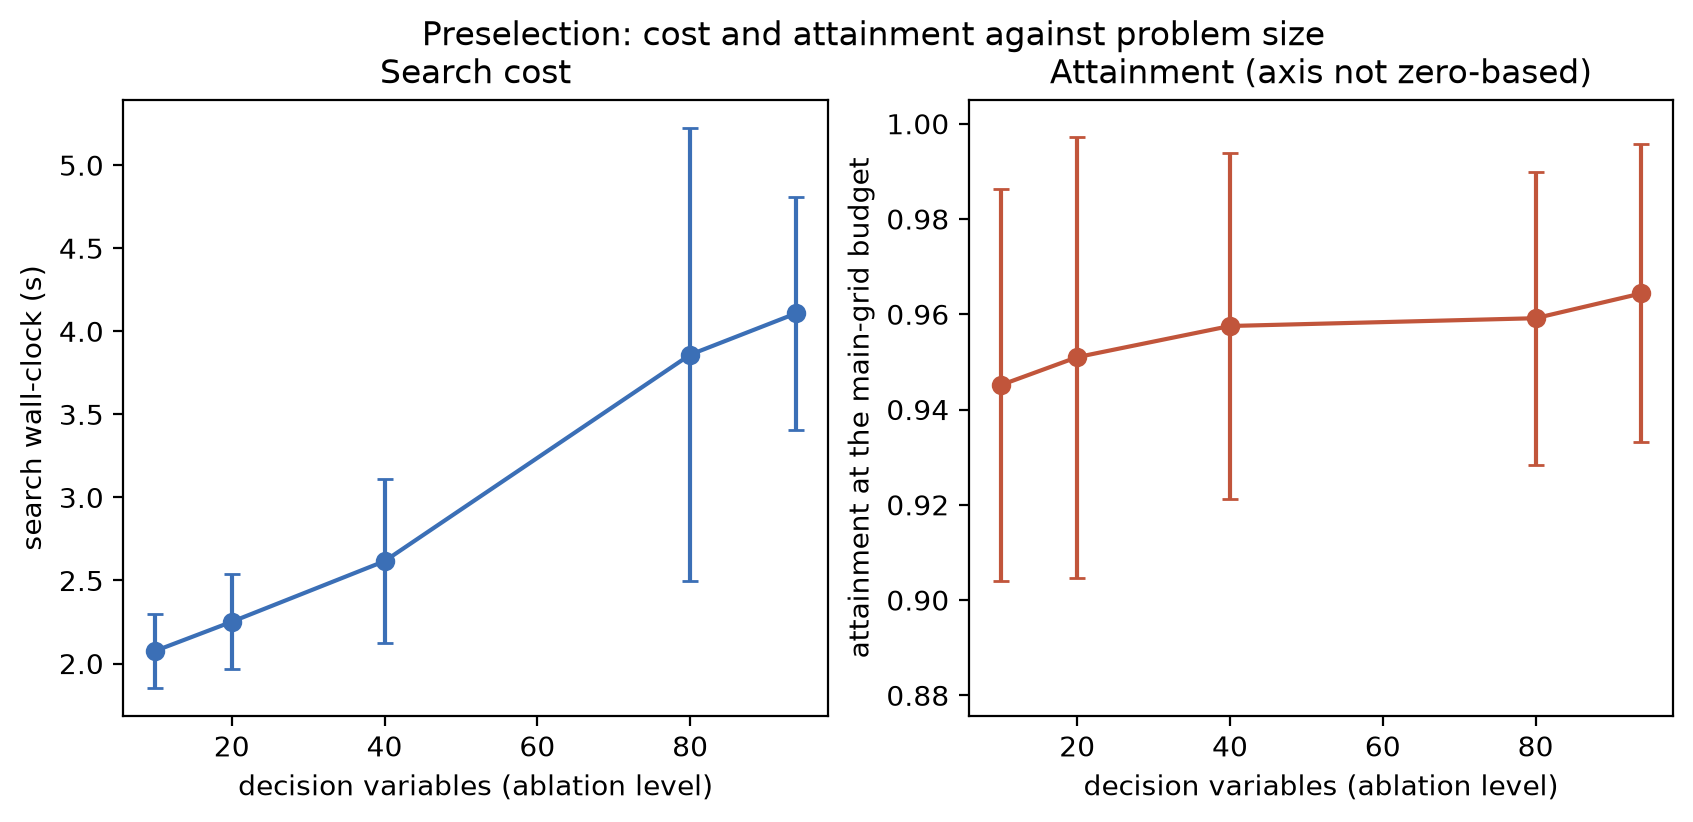
\includegraphics[width=\linewidth]{figures/fig_search_cost.png}
  \caption{Search cost and attainment against problem size, by ablation level, with standard deviations across seeds. The attainment axis is not zero-based. The rising attainment is the reading this paper argues is not interpretable on its own.}
  \label{fig:search-cost}
\end{figure}

\begin{figure}[htbp]
  \centering
  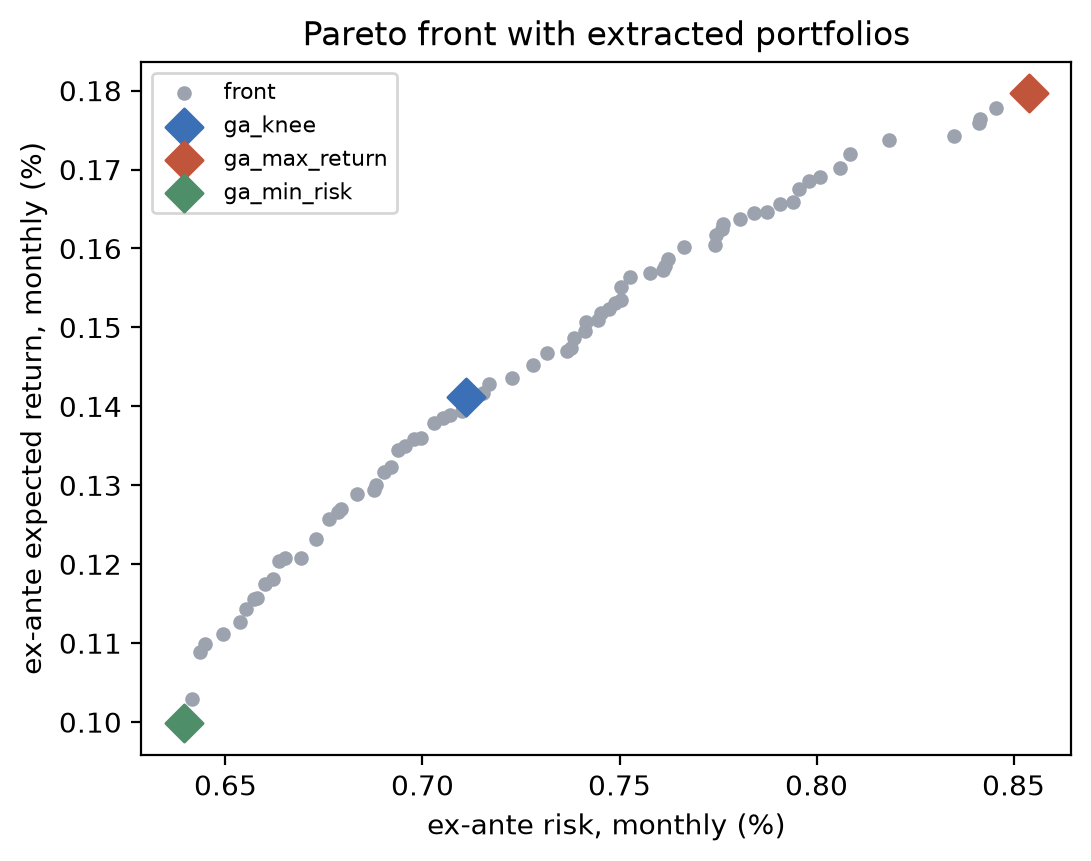
\includegraphics[width=\linewidth]{figures/fig_pareto_front.png}
  \caption{One Pareto front with the three extracted portfolios marked, at the median evaluation month under the no-screening control. The three profiles are nearly the same portfolio, which is the collapse reported in Section~\ref{sec:results} made concrete.}
  \label{fig:pareto}
\end{figure}

\begin{figure}[htbp]
  \centering
  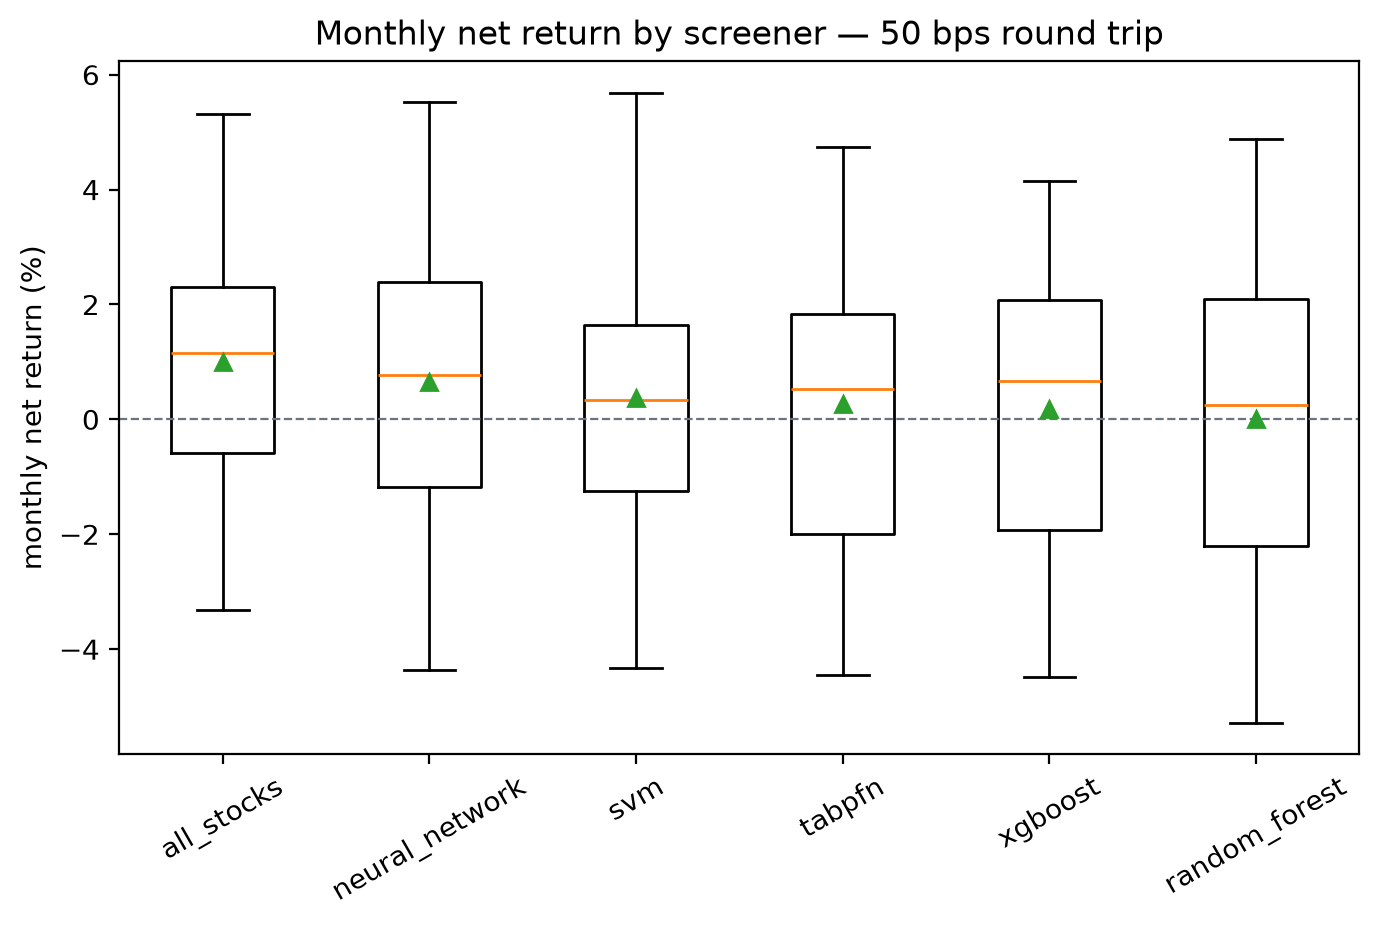
\includegraphics[width=\linewidth]{figures/fig_performance.png}
  \caption{Distribution of monthly net return by screening arm at the primary cost scenario.}
  \label{fig:performance}
\end{figure}

\begin{figure}[htbp]
  \centering
  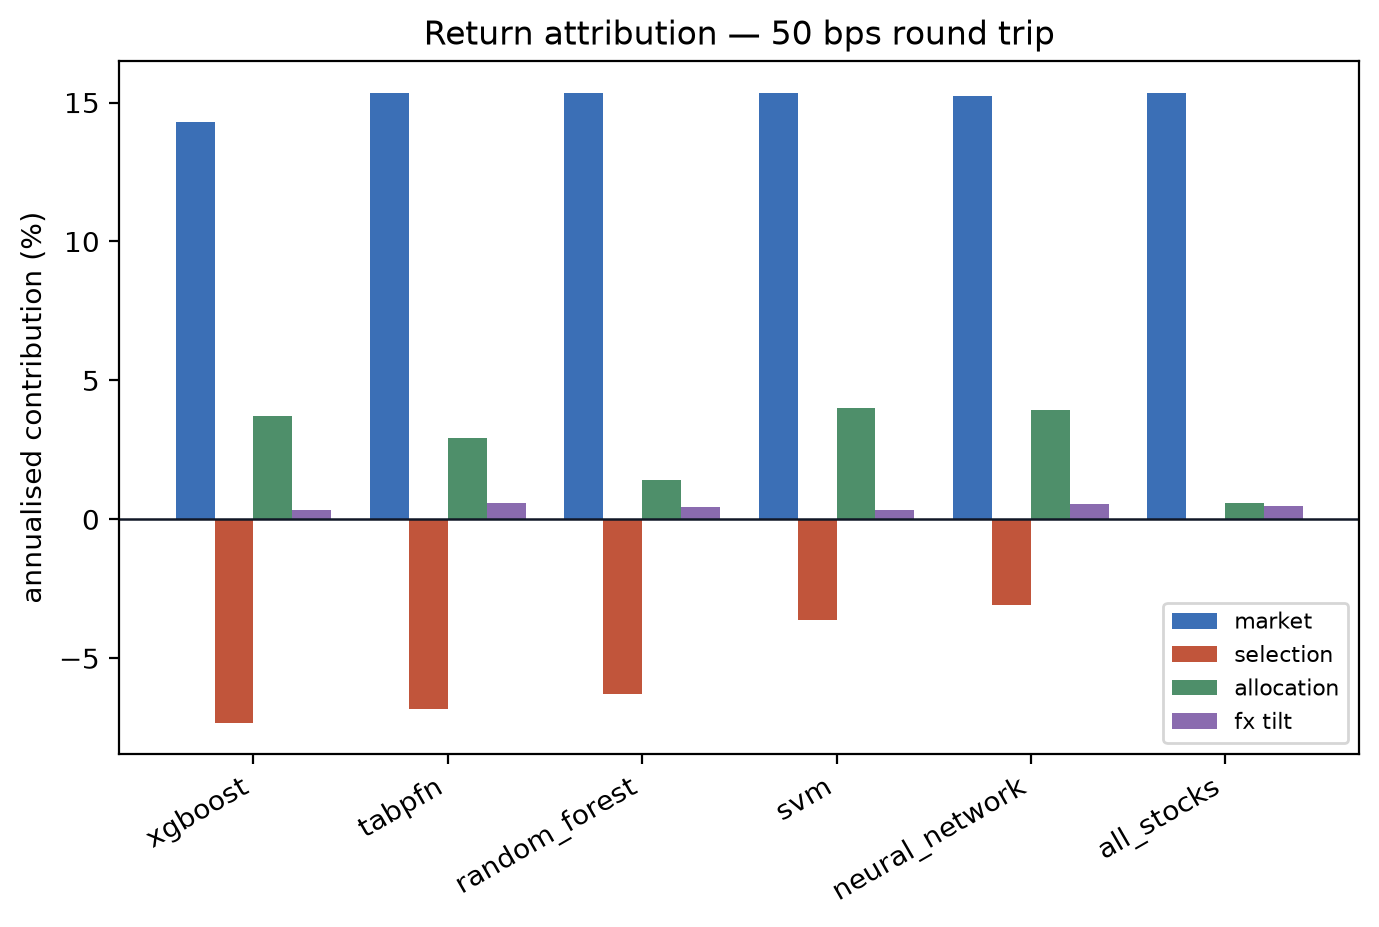
\includegraphics[width=\linewidth]{figures/fig_attribution.png}
  \caption{Return attribution by screening arm. The selection component is negative for every arm and exactly zero for the no-screening control, which validates the decomposition.}
  \label{fig:attribution}
\end{figure}

\begin{figure}[htbp]
  \centering
  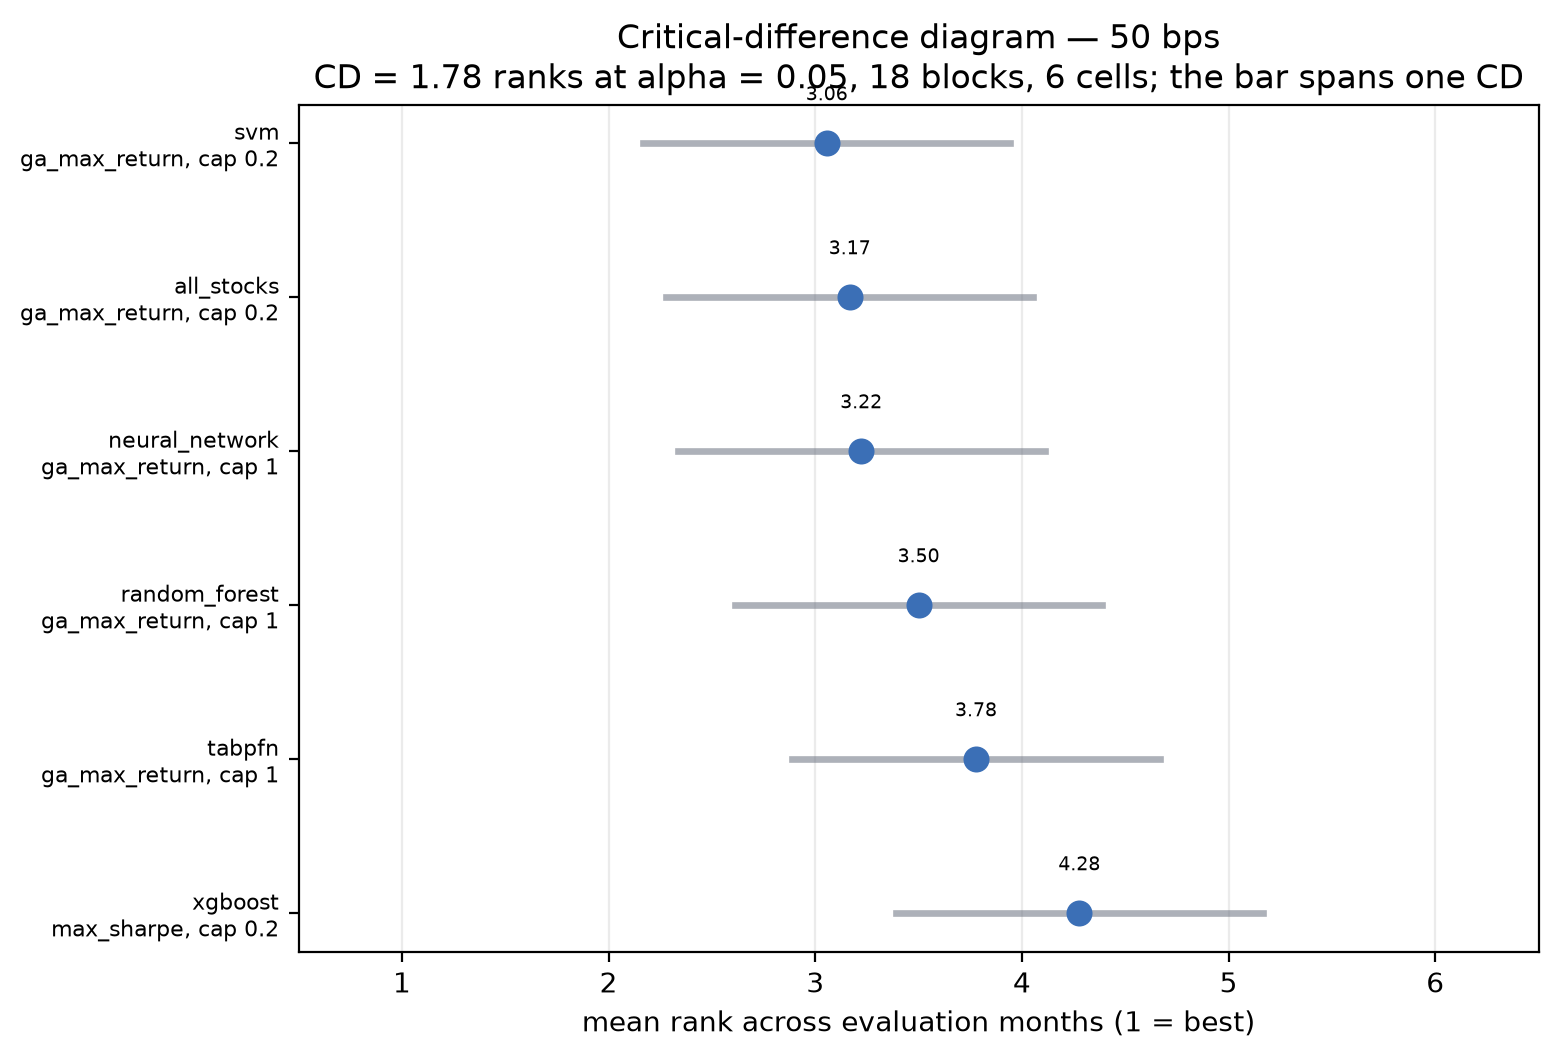
\includegraphics[width=\linewidth]{figures/fig_critical_difference.png}
  \caption{Critical-difference diagram over the pre-registered headline set. The bar spans one critical difference; no pair is separated.}
  \label{fig:critical-difference}
\end{figure}

\begin{table}[htbp]
  \centering
  \small
  \caption{Per-screener performance at the primary cost scenario.}
  \label{tab:performance}
  \begin{tabular}{lrrrrrrrr}
\toprule
screener & cost\_bps & net\_annualised & gross\_annualised\_upper\_bound & median\_sharpe & mean\_turnover & mean\_selection\_size & positive\_months & n\_blocks \\
\midrule
all\_stocks & 50.0000 & 0.1200 & 0.1591 & 0.8348 & 0.3196 & 93.8333 & 12 & 18 \\
neural\_network & 50.0000 & 0.0789 & 0.1624 & -0.3509 & 0.7123 & 32.6578 & 11 & 18 \\
svm & 50.0000 & 0.0441 & 0.1205 & -0.5810 & 0.6372 & 35.7407 & 10 & 18 \\
tabpfn & 50.0000 & 0.0319 & 0.1004 & -0.4716 & 0.6126 & 39.9815 & 10 & 18 \\
xgboost & 50.0000 & 0.0212 & 0.0966 & -0.5125 & 0.7017 & 33.2830 & 11 & 18 \\
random\_forest & 50.0000 & 0.0012 & 0.0834 & -0.8801 & 0.6738 & 32.6852 & 10 & 18 \\
\bottomrule
\end{tabular}

\end{table}

\begin{table}[htbp]
  \centering
  \small
  \caption{Every arm ranked against the comparator confrontation. No comparison resolves: the detectable bound exceeds every difference, as the notes record.}
  \label{tab:comparators}
  \begin{tabular}{llrrrrrrrlr}
\toprule
arm & tier & cost\_bps & net\_annualised & median\_sharpe & mean\_turnover & difference\_vs\_best\_proposed & p\_adjusted & minimum\_detectable\_annualised & verdict & reference\_series\_uncosted \\
\midrule
momentum\_equal\_weight & tier1 & 50.0000 & 0.2824 & 2.1397 & 0.2744 & -0.0311 & 1.0000 & 0.3870 & not rejected; effect below the design's resolution & False \\
bmv\_ipc & tier0 & 50.0000 & 0.1943 & NaN & 0.0000 & 0.0570 & 1.0000 & 0.5291 & not rejected; effect below the design's resolution & True \\
l4\_single\_objective\_ga\_sharpe & tier2 & 50.0000 & 0.1732 & 1.3710 & 0.3408 & 0.0780 & 1.0000 & 0.3062 & not rejected; effect below the design's resolution & False \\
equal\_weight\_universe & tier1 & 50.0000 & 0.1390 & 0.1751 & 0.0987 & 0.1122 & 1.0000 & 0.4083 & not rejected; effect below the design's resolution & False \\
proposed:all\_stocks & factorial & 50.0000 & 0.1200 & 0.8348 & 0.3196 & NaN & NaN & NaN &  & False \\
inverse\_volatility & tier1 & 50.0000 & 0.1036 & -0.2261 & 0.1004 & 0.1477 & 1.0000 & 0.4353 & not rejected; effect below the design's resolution & False \\
mv\_analytic\_universe & tier1 & 50.0000 & 0.0893 & -0.6446 & 0.2518 & 0.1620 & 1.0000 & 0.4804 & not rejected; effect below the design's resolution & False \\
sp500\_mxn & tier0 & 50.0000 & 0.0859 & NaN & 0.0000 & 0.1654 & 1.0000 & 0.3904 & not rejected; effect below the design's resolution & True \\
proposed:neural\_network & factorial & 50.0000 & 0.0789 & -0.3509 & 0.7123 & NaN & NaN & NaN &  & False \\
cetes\_28d & tier0 & 50.0000 & 0.0783 & NaN & 0.0000 & 0.1730 & 1.0000 & 0.4889 & not rejected; effect below the design's resolution & True \\
l6\_l1\_shrinkage\_mv & tier2 & 50.0000 & 0.0760 & -0.8789 & 0.2210 & 0.1753 & 1.0000 & 0.4881 & not rejected; effect below the design's resolution & False \\
proposed:svm & factorial & 50.0000 & 0.0441 & -0.5810 & 0.6372 & NaN & NaN & NaN &  & False \\
proposed:tabpfn & factorial & 50.0000 & 0.0319 & -0.4716 & 0.6126 & NaN & NaN & NaN &  & False \\
proposed:xgboost & factorial & 50.0000 & 0.0212 & -0.5125 & 0.7017 & NaN & NaN & NaN &  & False \\
proposed:random\_forest & factorial & 50.0000 & 0.0012 & -0.8801 & 0.6738 & NaN & NaN & NaN &  & False \\
\bottomrule
\end{tabular}

\end{table}

\begin{table}[htbp]
  \centering
  \small
  \caption{Return decomposition into market, selection, allocation and currency tilt.}
  \label{tab:attribution}
  \begin{tabular}{lrrrrrrrr}
\toprule
screener & cost\_bps & market\_annualised & selection\_annualised & allocation\_annualised & fx\_tilt\_annualised & portfolio\_sic\_weight & universe\_sic\_share & max\_abs\_residual \\
\midrule
all\_stocks & 50.0000 & 0.1535 & 0.0000 & 0.0058 & 0.0049 & 0.5165 & 0.5600 & 0.0000 \\
neural\_network & 50.0000 & 0.1524 & -0.0308 & 0.0392 & 0.0056 & 0.5277 & 0.5601 & 0.0000 \\
svm & 50.0000 & 0.1535 & -0.0363 & 0.0402 & 0.0032 & 0.5350 & 0.5600 & 0.0000 \\
random\_forest & 50.0000 & 0.1535 & -0.0627 & 0.0141 & 0.0044 & 0.5477 & 0.5600 & 0.0000 \\
tabpfn & 50.0000 & 0.1535 & -0.0682 & 0.0294 & 0.0059 & 0.5275 & 0.5600 & 0.0000 \\
xgboost & 50.0000 & 0.1431 & -0.0732 & 0.0372 & 0.0032 & 0.5337 & 0.5597 & 0.0000 \\
\bottomrule
\end{tabular}

\end{table}

\begin{table}[htbp]
  \centering
  \small
  \caption{The three investor profiles, each against its designated metric.}
  \label{tab:profiles}
  \begin{threeparttable}
\small
\setlength{\tabcolsep}{4pt}
\begin{tabularx}{\linewidth}{>{\raggedright\arraybackslash}Xllrr}
\toprule
Profile & Metric & Screening arm & Value & Annualised \\
\midrule
aggressive & return net & all stocks & 0.01 & 16.4\% \\
aggressive & return net & neural network & 0.01 & 13.7\% \\
aggressive & return net & random forest & 0.00 & 3.8\% \\
aggressive & return net & svm & 0.01 & 16.1\% \\
aggressive & return net & tabpfn & 0.00 & 1.1\% \\
aggressive & return net & xgboost & 0.00 & 4.3\% \\
conservative & sigma realized & all stocks & 0.01 & -- \\
conservative & sigma realized & neural network & 0.01 & -- \\
conservative & sigma realized & random forest & 0.01 & -- \\
conservative & sigma realized & svm & 0.01 & -- \\
conservative & sigma realized & tabpfn & 0.01 & -- \\
conservative & sigma realized & xgboost & 0.01 & -- \\
moderate & sharpe & all stocks & 1.01 & -- \\
moderate & sharpe & neural network & 0.55 & -- \\
moderate & sharpe & random forest & -0.49 & -- \\
moderate & sharpe & svm & 0.12 & -- \\
moderate & sharpe & tabpfn & -0.02 & -- \\
moderate & sharpe & xgboost & -0.24 & -- \\
\bottomrule
\end{tabularx}
\begin{tablenotes}[flushleft]\footnotesize
  \item cost bps: 50.00 -- Blocks: 18
\end{tablenotes}
\end{threeparttable}

\end{table}


% --- screening_justification ---------------------------------------------
\section{Does preselection justify itself?}\label{sec:screening-justification}

The original formulation motivates supervised screening on two grounds: that it improves the portfolio by removing instruments predicted to fall, and that it makes the optimisation tractable by reducing the number of decision variables. The ablation tests both, over 450 instances spanning 10 to 94 decision variables with no-preselection as an explicit level.

\textbf{On portfolio quality, the argument fails.} The no-screening control returns 12.0\% annualised against 7.9\% for the best screening arm, a gap of 4.1\%. The gap is below the design's resolution and is therefore not a significant difference, but it points the wrong way for the method, and the attribution decomposition shows why: the selection component is negative for every screener.

\textbf{On computational cost, the argument also fails, and by a wide margin.} Wall-clock rises from 2.1 to 4.1 seconds between 10 and 94 variables -- a factor of 2.0 -- while the covariance matrix grows by a factor of 88. The quadratic growth in problem size does not translate into a proportionate cost, so preselection is not buying compute.

\textbf{On tractability, the argument holds, and this study initially missed it.} The obvious metric says otherwise: attainment against an extended-budget reference rises with problem size. That metric is self-referential, because the reference front comes from the same optimiser. Against the closed-form attainable range -- maximum return is the whole budget in the highest-mean asset, minimum variance is analytic -- the picture inverts. Return coverage falls from 61.3\% at 10 variables to 10.2\% at 93; risk coverage falls from 34.0\% to 4.3\%. The search genuinely degrades with dimension.

The two findings are separable and both are reported. Preselection does make the optimisation easier in a way that is real and measurable. It does not follow that preselection helps, because the screening signal is negative enough to outweigh what the smaller search space buys. A reader who wants the tractability benefit without the selection penalty should look at dimension reduction that does not condition on a predicted return.


% --- limitations ---------------------------------------------------------
\section{Limitations}\label{sec:limitations}

\textbf{Resolution.} Conclusions rest on 18 monthly blocks, giving a minimum detectable effect of 12.7\% to 17.1\% annualised. No factor effect in the study exceeds that bound. The hierarchical Friedman tests return p between 0.42 and 0.68, and the critical difference over the headline set is 1.78 ranks against a spread far smaller. These are statements about the design, not about the world, and a longer window is the single change that would most improve the study.

\textbf{Dependence and the mixed model.} Fitting the mixed model over 21,275 cell-months yields standard errors between 6 and 9 times smaller than resampling whole months, because cells within a month hold overlapping stocks and a single random intercept removes only the month's common level. The point estimates agree; the apparent significance does not survive. The month-paired tests are confirmatory, as pre-registered, and the model is reported as descriptive. The labeling-by-allocator interaction -- the direct test of whether an apparent labeling advantage is really a concentration effect -- has 10 terms and none reaches significance even at the model's inflated precision.

\textbf{Survivorship.} The universe is screened point-in-time from price history rather than from an exchange listing record, because the exchange's listing endpoints were unavailable and no archived snapshot exists. No instrument ceased trading during the evaluation window. That is a lower bound on the exposure, not a proof of its absence.

\textbf{Costs.} Transaction costs are applied after optimisation rather than inside the objective, so the optimiser never trades return against the cost of achieving it. Costs are also charged at a flat spread across instruments. Real spreads widen on the smaller and less liquid names, which the screening arms select more often than the control does, so the flat assumption flatters the screened arms relative to the control -- the bias runs against the study's own conclusion rather than toward it.

\textbf{Covariance estimator.} The shrinkage sensitivity arm moves the reported contrasts by at most 0.7\% annualised and no contrast reverses sign. The arm covers a subset of screeners and one labeling strategy, so this is an argument from the observed effect size rather than a proof of insensitivity across the full grid.

\textbf{Scope.} The study covers one exchange over one window with one feature dictionary. Nothing here establishes that supervised screening subtracts value in general; it establishes that it did so here, under a protocol designed in advance to be able to detect the opposite.


% --- conclusions ---------------------------------------------------------
\section{Conclusions}\label{sec:conclusions}

An indicator computed against a reference the system produced itself cannot detect a failure the system makes consistently. We gave a case where this is not a theoretical concern: on a constrained portfolio problem, attainment against an extended-budget reference rises with problem size while coverage against the closed-form attainable range falls by a factor of roughly six, and the two readings support opposite conclusions about whether preselection is needed for tractability.

The correction is cheap where it applies. Coverage requires only that each objective's extreme be computable alone, which holds for a wide class of constrained formulations, and it is bounded, normalised and immune to any bias the produced and reference fronts share. We recommend it be reported alongside attainment rather than instead of it, and we give the condition -- high attainment beside low coverage -- under which an attainment figure should not be believed.

For the system studied, the diagnostic separated two claims that are usually made together. Supervised preselection does make the search easier, measurably and in the direction its proponents assert. It does not improve the portfolio: no screening arm beat passing the whole admitted universe to the optimiser, and return attribution located the shortfall in a negative selection component present in every arm. A practitioner who wants the search benefit should seek it from dimension reduction that does not condition on a predicted return.

We are explicit about what this study cannot settle. 18 evaluation blocks give a detectable effect of 12.7\% to 17.1\% annualised, and no effect we estimated exceeds it, so the performance comparisons are unresolved rather than null. The coverage result does not depend on that bound: it is a measurement against a computed quantity, replicated across months and seeds, and its direction is unambiguous.


% --- future_work ---------------------------------------------------------
\section{Future work}\label{sec:future-work}

\textbf{Cost-aware optimisation.} The most direct extension is to move transaction costs inside the objective rather than applying them afterward. Realised turnover is high enough that the optimiser is currently choosing portfolios it would not choose if it were charged for reaching them, and a third objective or a turnover penalty would let the front express that trade-off rather than have it imposed after the fact.

\textbf{Search that reaches the extremes.} The coverage result gives a concrete target: at 93 decision variables the optimiser spans 10.2\% of the attainable return range. Reference-direction methods, decomposition-based algorithms, or simply seeding the population with the analytic extremes would attack this directly, and the closed-form bound gives an unambiguous measure of progress that attainment against a self-produced reference cannot provide.

\textbf{Dimension reduction without return prediction.} The ablation separates a real tractability benefit from a harmful selection signal. Clustering, sector-balanced sampling, or liquidity-based admission would reduce the search space without conditioning on a predicted return, and would test whether the benefit survives when the penalty is removed.

\textbf{Longer windows and more blocks.} The design's resolution is the binding constraint on every conclusion. Extending the evaluation window is the change that most improves what can be claimed, and the protocol is specified so that this requires no methodological change.

\textbf{Alternative labels.} All three labeling strategies condition on realised returns over a one-month horizon. Labels defined on risk-adjusted outcomes, on longer horizons, or on relative rather than absolute performance would test whether the negative selection component is a property of supervised screening or of this particular target.

\bibliographystyle{elsarticle-harv}
\bibliography{references}

\end{document}
